%!TEX root = ../main.tex
%=========================================================

\section{Design}
\label{sec:design}

In the following, we provide an overview of the design and the objectives of \textit{i)} register operations at a single registrar, followed by \textit{ii)} the process of distributing ads and performing search across multiple registrars in the network. Finally, we discuss the process of search and establishing sub-protocol connections. 

\subsection{Topic registration with a single registrar}

Central to the registration process is the topic table. Below, we provide a description of the topic table, followed by the registration process with a single registrar. 

\subsubsection{Topic Table}

Registrars store advertisers ads locally in a data structure called \emph{topic table}, 
indexed by advertisement topic. 
Each list of ads for a particular topic in the table  can be considered as a \emph{topic queue} because it functions like a FIFO queue.
Ads enter the queue once the registrar ticket is accepted,  and
the ad remain in the queue for a constant amount of time \texttt{target-ad-lifetime}. 
When \texttt{target-ad-lifetime} expires the ad is removed  from the queue.

\begin{figure}
    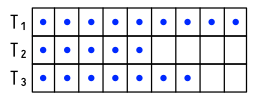
\includegraphics[width=0.35\textwidth]{img/topic-queue-diagram.png}
    \caption{Topic table structure.}
    \label{fig:topic_table}
 \end{figure}

The total size of the topic table is limited by \texttt{topic table capacity},  however there is no per-topic limits since existing number of topics in the network is unknown. 
Reasonable \texttt{topic table capacity} is 50,000 ads. 
Since ENRs are at most 300 bytes in size, these limits ensure that a full topic table consumes approximately 15MB of memory.
An advertiser can only place a single ad for a specific topic queue in the topic table at the same time; duplicate placements are rejected (although the same node may attempt placing ads for multiple topics at the same registrar).

The topic table is shared across multiple advertisers and stores topics with varying popularity (which is determined by how many nodes register the topic) among the participants of Discv5. 
It is important that the high popularity of a particular topic should not prevent peers from registering less popular topics. 
This is achieved using the waiting time function that will determine the time an advertiser will have to wait to place an ad after a ticket request,  and is detailed in Section~\ref{sec:waitingTime}.

\subsubsection{Registration Procedure}

In order to place an ad on a registrar's topic table, the advertiser must present a valid 'ticket' to the registrar. Tickets are immutable objects issued by the registrars. An advertiser willing to register an ad at a registrar must first obtain a ticket from that registrar by sending a 'ticket request' (TICKETREQUEST) message to the registrar. In response to the ticket request, the registrar issues an initial ticket containing a 'waiting time' and sends the ticket to the advertiser in a 'ticket response' message. The advertiser can come back to the registrar (to register an ad) after the waiting time has elapsed and present the ticket in a 'topic registration request' (i.e., REGTOPIC) message.

Any REGTOPIC messages that are sent before the waiting time (indicated in the ticket) are ignored by the registrars. If the advertiser comes back to the registrar after the waiting time, the advertiser can either place the ad (and notify the advertiser of a successful registration) or issue another ticket with a new waiting time in another ticket response message. An advertiser may be given one or more tickets in a sequence before a successful registration, and this means that overall the advertiser waits for a 'cumulative waiting time' period that is the sum of multiple waiting times issued in each ticket in the sequence before finally registering an ad. Assignment of 'waiting times' is the only way the registrars can control the registrations in order to both:

\begin{itemize}
    \item Throttle ad placement rate to prevent overflowing of topic table: when the topic table is full, the advertisers must wait for already placed ads to expire first before they are allowed to register new ads.
    \item Prioritise registrations to achieve a diverse set of ads in the topic table. For example, registrations for less popular topics or registrations from advertisers that increase IP diversity (in the set of advertiser IP addresses that currently have an ad in the table) can be prioritised over others. This is useful to reduce the impact of Sybil attacks on the service discovery system.
\end{itemize}

Waiting times will be calculated according to a 'Waiting time function' (see below). Enforcing this time limit prevents misuse of the topic table because any topic must be important enough to outweigh the cost of waiting for ad placement. Imagine a group phone call: announcing the participants of the call using topic advertisement isn't a good use of the system because the topic exists only for a short time and will have very few participants. The waiting time prevents using the topic table for this purpose because the call might already be over before everyone could get registered. Also, it prevents attackers from overflowing topic table by regulating registrations in case of spamming attacks.

In addition to the waiting time,  the sequence of tickets issued by a registrar for a specific advertiser also records the original issue-time of the first ticket which can be used to compute the cumulative waiting time so far; that is, the time elapsed since the advertiser requested its first ticket to place its ad. The inclusion of issue-time allows the registrars to prioritise advertisers that have been waiting the most as we explain later. Because the tickets are immutable (i.e., tampering with the ticket is detectable by the registrars that originally issued the ticket), when a registrar issues a new ticket (in case a registration is not immediately successful) to an advertiser, the registrar simply copies the issue-time from the last issued ticket and use that as the issue-time of the new ticket. This means that the registrars are not required to maintain any state for each on-going ticket request given that they can simply verify the authenticity of the ticket in the incoming registration requests. The registrars ensure the authenticity of the tickets they issue to the advertisers through symmetric encryption we explain below.

Tickets are immutable objects storing arbitrary information determined by the issuing registrar node.  While details of encoding and ticket validation are up to the implementation, tickets must contain enough information to verify that:
\begin{itemize}
    \item The advertiser attempting to use the ticket is the one which originally requested it.
    \item A ticket is valid for a single topic only.
    \item A ticket can only be used within the 'registration window' (explained below).
    \item A ticket can not be used more than once. \michal{Can we enforce it? I can use the same ticket twice within the validity period, right?\onur{It seems possible for an advertiser to essentially duplicate an existing ticket by using it twice during the validity period. The duplicate ticket gets a new waiting time, accumulates a high cum. waiting time so that the advertiser can re-register its ad with significant advantage over other contenders. I think an easy fix is for registrars to drop/ignore tickets for which there is an active registration. }}
\end{itemize}

Tickets cannot be used beyond their lifetime. If an advertiser does not come back after the waiting time, all cumulative waiting time is lost and the advertiser must start over (\Cref{fig:ticket_validity}). When the ticket is issued, the node keeping it must wait until the registration window opens. The length of the registration window is implementation dependent, but by default 10 seconds is used. The ticket becomes invalid after the registration window has passed. This mechanism prevents malicious advertisers from obtaining a ticket, then just wait for a long time until a large cumulative waiting time is accumulated, and finally launch a coordinated attack to take over the topic table with their ads.
    
\begin{figure}
    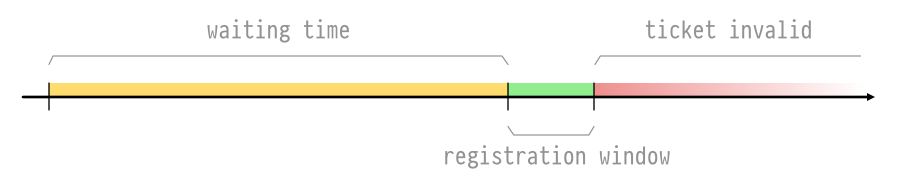
\includegraphics[width=0.5\textwidth]{img/ticket-validity}
    \caption{Ticket validity period.}
    \label{fig:ticket_validity}
\end{figure}

\subsection{Distributing ads across registrars}

The above description explains the storage and placement of ads on a single registrar, but the advertisers need to distribute ads redundantly on multiple nodes in order to speed up its discovery and to be discovered by more searchers at once. 
The main goal of distributing advertisements to be found within the network. An important issue is how advertisers distribute their ads among registrar nodes. 
Since every node may act as an advertisement medium for any topic,  advertisers and searchers looking for ads must somehow meet at common registrars. 
Ideally, the topic search should be fast even when the number of advertisers for a topic is much smaller than the number of all live nodes. Given that in a decentralised setting, advertisers and registrars can not apriori agree on a subset of nodes to serve as the advertisement media for the topics, the main challenge for nodes is to find the "right" set of nodes to send advertisements and topic search queries so that they quickly meet at common nodes.

In order to execute the ad distribution process described below,  each advertiser maintains a per-topic 'ticket table' for each topic it is advertising to keep track of the ongoing registration attempts with different registrars. 
This table is similar to the routing table used in Kademlia protocol, but instead of storing nodes based on distance for routing purposes, nodes are stored based on distance to topic ID to keep track of on-going registrations.

This table is made up of k-buckets of logarithmic distance to the topic hash (topic ID), i.e. the table stores k registrars for every distance step (bucket). It is sufficient to use a small value of k such as k=3. 
%For this table no replacement list is used, different from the Kademlia routing table. 
Ticket table buckets are initially filled from the local routing table (Kademlia DHT Table) with the same distance to the topic hash.

Every node stored in the ticket table is a potential registrar. The advertiser attempts to place an ad on each registrar and keeps the latest ticket issued by that registrar. It also keeps references to all pending tickets in a priority queue keyed by the expiry time of the ticket so it can efficiently access the next ticket for which a placement attempt is due.

In our approach, advertisers start a limited number of parallel registrations in each ticket table bucket distance. More specifically, an advertiser follows the below steps to distribute its ads for a specific topic:
\begin{enumerate}
        \item The advertiser (\hl{randomly?}) selects a set of K registrar nodes from each bucket distance of the ticket table structure, where the number of bucket distances (B) is a configurable parameter of the ticket table.
    \item A TICKETREQUEST message is initially sent to each of the selected registrar nodes in the previous step.
    \item Registrar node replies with a TICKETRESPONSE. This message includes the TICKET which contains a waiting time and a ticket issue time.
    \item The advertiser replies after the waiting time expires with a REGTOPIC request containing the previously received TICKET attached to it.
    \item A registration is successful when the waiting time calculated at the registrar is smaller than the cumulative waiting time, which means that the advertiser has waited long enough.
    \item The registrar sends a REGCONFIRMATION response to the advertiser of the successful registration. In general, the topic table occupancy is guaranteed to always remain below the topic table capacity by the waiting time calculated: the waiting time function returns increasingly large values as the topic table space runs out; the waiting time becomes infinite in case there is no space.
    \item The registrar replies with a REGRESPONSE message containing a new TICKET (containing a new waiting time) in case the registration is not successful.
    \item A registrar gives up and stops the registration process with a registrar (say R) upon either T unsuccessful registration attempts (i.e., after being issued T tickets in REGRESPONSE messages from the registrar without a REGCONFIRMATION) or receipt of a ticket with a waiting time larger than LARGEWAIT. In that case, the advertiser selects a new node located in the same bucket as R, and initiates a TICKETREQUEST (step 2).
    \item Similarly, expiration of a previously placed ad (i.e., after the passage of ad-lifetime upon receiving a REGCONFIRMATION message) also triggers TICKETREQUEST to a new (\hl{why not the same node?}) node that is in the same bucket as R.
\end{enumerate}

The objective of the ad placement process described above is to establish and maintain K active (i.e., unexpired) registrations in each bucket distance. This objective is achieved by the advertisers setting a timer with a duration of ad-lifetime immediately upon the receipt of a REGCONFIRMATION from a node in a bucket b, and once the timer expires (after ad-lifetime passes) the advertiser starts a fresh registration with a node that is also located in bucket b. The ticket table is used to store the tickets obtained for each on-going registrations and to keep track of the expiration times of active registrations.

%\subsubsection{Bucket refresh}

The Ticket table needs to be initialised and refreshed to fill up all the per-distance k-buckets. 
Ideally,  all k-buckets should be constantly full,  meaning that the advertisers place registrations at registrars in all distances to the topic hash. 
An option to fill up all k-buckets would be to send periodic lookups for the specific distance to the topic hash, but since there are some distances that tend to be empty in the id space,  sending periodic lookups for the topic hash may create an additional overhead that can be too expensive and create too much traffic in the network. To avoid that, initially, the 'ticket table' k-buckets are filled performing local Kademlia routing table lookups to all distances to the 'topic hash' of the advertised topic.

In addition to that, every time a node sends a ticket or registration request, the registrar replies with the closest nodes to 'the topic hash' that it knows. This helps filling up k-buckets without sending additional lookups. 
Also, when performing topic search (sending lookups for specific topics),  closest known nodes to 'the topic hash' are attached by the registrar node in the response.

There is  a refresh bucket process, similar to the Kademlia DHT table,  where periodically a random bucket is checked to see if it is empty.
The \texttt{refresh time} is a configurable parameter. 
We set a \texttt{refresh time=10 seconds} as a reference for our performance evaluation.
During the refresh process,  in case the bucket checked is empty, 
a local lookup to the Kademlia DHT table is performed. 
In case no nodes have been found for the bucket distance,  a Kademlia lookup is performed towards the topic hash~\footnote{The lookup is performed by sending a FINDNODE message,  as described inhttps://github.com/ethereum/devp2p/blob/master/discv4.md.}
Also, all nodes in the checked bucket are pinged to check they are still alive. 
In case they are not, tickets for those dead nodes are removed from the ticket table and registrations to new nodes are initiated.

\subsection{Topic Search}

The purpose of placing ads is to be discovered by other nodes interested in the same topic.  
Searcher nodes maintain a separate table that they use to keep track of on-going searches called the \emph{search table}. 
Similar to the \emph{ticket table}, the search table also stores k-buckets of registrar nodes by distance to the topic hash and buckets are initially filled from the local routing table (Kademlia DHT Table) with the same distance to the topic hash.
Also,  every time an advertiser sends a ticket request and when performing topic search at a registrar,  when registrar replies with the closest nodes to 'the topic hash' that it knows,  nodes are stored in the \emph{search table} helping filling up all k-buckets.
For each topic the client wants to start discovering nodes, a new \emph{search table} is created. 
%and a new 'search table' is created for each topic. 
The bucket size \texttt{k}  of the search table should be relatively large in order to make the search efficient. 
By default we use\texttt{k=16},  similarly to the local routing table (Kademlia DHT).
Tickets are not required for search and nodes can not be added multiple times in the same k-bucket.

\subsubsection{Search Procedure}

To find ads,  the searcher simply queries the nodes in the search table for ads. 
During lookup process \texttt{ALPHA} parallel lookups are performed to three different nodes. 
\texttt{ALPHA} is the parameter that establishes how many lookup messages are sent in parallel, and by default is set to \texttt{3}.
In case not enough results have been received for the first ALPHA lookups,  additional ALPHA parallel lookups are performed until
reaching the goal of number of discovered node per topic.
This is also a configurable parameter names \texttt{LOOKUP\_LIMIT} and by default is set to \texttt{50 nodes}. 
In case  \texttt{LOOKUP\_LIMIT}  is not reached, the lookup process is stopped after a maximum number of hops. 
\texttt{MAX\_LOOKUP\_HOPS} is established to set to number of hops limit, and is set to 50 by default.
Once  \texttt{LOOKUP\_LIMIT} or \texttt{MAX\_LOOKUP\_HOPS} is reached,  all nodes discovered for the queried topic are sent to the client to start establishing connections with the nodes.
After trying connections with all nodes,  subsequent lookups are performed in case is necessary to discover additional nodes.

We implemented and evaluated a lookup strategy that choose which nodes from which buckets ask first trying to diversify the nodes discovered as much as possible and trying not to overload nodes close the topic hash.
A random node is picked from a bucket following a round-robin approach. 
It starts picking a random node from the highest distance bucket and follows to the next distance in the bucket list.
In order to find new results,  bucket entries are replaced when the node fails to answer or when it answers with an empty list of ads. 

There is also a refresh process,  equivalent to the \emph{ticket table} refresh process, where random buckets are selected and all nodes in the buckets are checked for liveness.
In case the bucket is empty a Kademlia lookup is performed towards the topic hash.

\subsubsection{Updating connections}

Using the search results, a searcher updates its subprotocol-specific connections. 
\onur{need to explain this process since security depends on that.}

%All the modifiers from the first part of the equation increase with increasing number of the same items that are already in the table, i.e., reduction in diversity. Thus it's getting increasingly difficult to register ads for the same IP/ID/topic. For instance, ads for less popular topic will receive lower waiting times than popular ones. Note that the table does not prevent anyone from registering, but rather makes it slower for already popular items. Such a mechanism promotes diversity in the table and protects against Sybil attacks so that an attacker who is in control of a limited pool of IP addresses won't be able to dominate the table with many ads. The low exponent for the topics is motivated by the topics in the network that are likely to follow a skewed (e.g., a zipf-like) distribution. In contrast, honest nodes' IPs/IDs should follow a uniform distribution.

%The latter part of the formula is determined based on a multiple of ad-lifetime and the current utilisation (i.e., occupancy divided by capacity) of the table. When the utilisation becomes closer to 1.0, the base time becomes very large due to a very small denominator. Before the waiting time becomes infinite (when utilisation becomes 1), the waiting time becomes extremely high, in which case the advertisers give up as explained in the ad distribution process.
